\documentclass{beamer}
\usepackage{multicol}
\usepackage{natbib} 
\def\newblock{\hskip .11em plus .33em minus .07em}
\newcommand\independent{\protect\mathpalette{\protect\independenT}{\perp}} 
\def\independenT#1#2{\mathrel{\rlap{$#1#2$}\mkern2mu{#1#2}}} 
%\usepackage{beamerthemeBerkeley}
% Use either the one above or the one below
\usetheme{Hannover}

\title{The Bootstrap}
%\author{	F. Daniel Hidalgo\\ }
%\date{\today}

\begin{document}

\frame{\titlepage}

%\section[Outline]{}
%\frame{\tableofcontents}

%Sample median
%bias
%hypothesis test
%confidence intervals

%regression
%parametric, non-parametric

%loess
%time series
\section{Sample Mean}

\frame{
	\frametitle{The Sample Mean and the Sample Median}
        \begin{itemize}
          \item Let $X_i$ be IID for $i=1,...,n$, with mean $\mu$ and
            variance $\sigma^2$. We use the sample mean $\bar X$ to
            estimate $\mu$.
            \item Is the estimator biased? What is it's standard
              error?
            \item Of course, we know it's unbiased and the SE is
              $\sigma/\sqrt{n}$, where $\hat \sigma^2 =
              \frac{1}{n}\sum_{i=1}^n(X_i - \bar X)^2$
            \item What about the median, particularly the difference
              in medians? Except for special circumstances, we don't
              have closed-form formulas for the uncertainty associated
              with these quantitites. 
            \end{itemize} 
}




\frame{
	\frametitle{The Bootstrap Algorithm for estimating standard
          errors}
        \begin{enumerate}
        \item Select $B$ independent bootstrap samples
          $\mathbf{x^{*1},x^{*2},...,x^{*B}}$, each consisting of $n$
          data values draw \textbf{with replacement} from $x$.
        \item Evaluate the bootstrap replication corresponding to each
          bootstrap sample, 
$$\hat \theta^*(b) = s(\mathbf{x^{*b}}) \qquad b=1,2,\ldots,B.$$
        \item Estimate the $\textrm{se}_F(\hat \theta)$ by the sample
          standard deviation of the $B$ replications
$$
\widehat{\textrm{se}}_B =\left \{ \sum_{b=1}^B[\hat \theta^*(b) - \hat
\theta^*(\cdot)]^2/(B-1)\right \}^{1/2};
$$
where $\theta^*(\cdot) = \sum_{b=1}^B \hat \theta^*(b)/B$
        \end{enumerate}
}

\frame{
	\frametitle{The Bootstrap Algorithm for SE}
     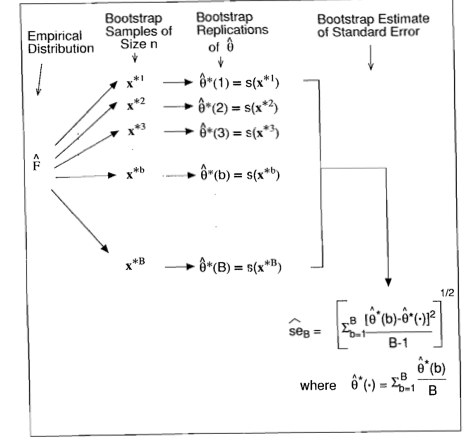
\includegraphics[width=8cm]{bootstrap_algorithm_se.png}  
}

\frame{
	\frametitle{The Plug-in Principle}
        \begin{itemize}
        \item We observe a random sample of size $n$ from a
          probability distribution $F$,
$$F \rightarrow (x_1,X_2,\ldots,x_n)$$
the empirical distribution function $\hat F$ is defined to be the
discrete distribution that puts probability $1/n$ on each value
$x_1,i=1,\ldots,n$.
\item The plug-in estimate of a  parameter $\theta = t(F)$ is defined
  to be $\hat \theta = t(\hat F)$.
        \end{itemize}
}

\frame{
	\frametitle{Confidence Intervals}
        \begin{itemize}
        \item Standard confidence intervals depend on the large sample
          or asymptotic result: 
$$\frac{\hat \theta  - \theta }{\hat{\textrm{se}}} \ensuremath{\sim}
N(0,1)$$
      \item In finite samples, we may not want to rely on that result
        and we instead can use bootstraped confidence intervals.
              \end{itemize}
}

\frame{
	\frametitle{Percentile Method}
\begin{itemize}
      \item Many methods of bootstraped confidence intervals, but the
  \textbf{percentile} method is probably the easiest and most
        intuitive.
      \item To proceed we generate $B$ independent bootstrap data
        sets $\mathbf{x^{*1}},\mathbf{x^{*2}},\ldots,\mathbf{x^{*B}}$
        and compute the bootstrap replications $\hat \theta^*(b) =
        s(\mathbf{x}^{*b})$ for $b=1,2,\ldots,B$.
      \item Let $\hat \theta^{*(a)}_B$ be the $100\cdot \alpha$th 
        empirical percentile of the $\hat \theta^*(b) $ values, that
        is the $B \cdot \alpha$th value in the ordered list of $B$
        replications of $\hat \theta^*$. Likewise let the $\hat
        \theta^{*(1-a)}_B$ be the $100\cdot  (1-\alpha)$th empirical percentile.
      \item The approximate $1-2\alpha$ percentile interval is 
$$[\hat \theta_{\%,lo},\hat \theta_{\%,up}] = [\hat \theta^{*(a)}_B,\hat \theta^{*(1-a)}_B] $$
\end{itemize}
}



\frame{
	\frametitle{Regression Models}
        \begin{itemize}
        \item Suppose $Y=X\beta + \epsilon$, where the design matrix
          is $n \times p$, $X$ is fixed and has full rank. The
          parameter vector  $\beta$ is $p\times1$, unknown, to be
          estimated by OLS. The errors $\epsilon_1,\ldots,\epsilon_n$
          are IID with mean 0 and variance $\sigma^2$.
        \item If we forgot the formulas and wanted to estimate the
          bias and variance of OLS, we could use the bootstrap. What's
          random here?
        \item In the model, the $Y_i$'s are random, but not IID. The
          $\epsilon_i$ are random and IID but unobserved. What do we do?
        \item We can re-sample the residuals: $e = Y- X\hat \beta$. 
        \end{itemize}
     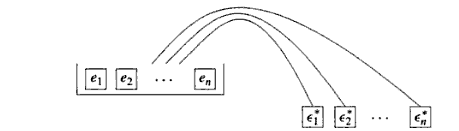
\includegraphics[width=8cm]{bs_reg.png}  
}

\frame{
	\frametitle{Regression Models}
        \begin{itemize}
        \item Suppose $Y=X\beta + \epsilon$, where the design matrix
          is $n \times p$, $X$ is fixed and has full rank. The
          parameter vector  $\beta$ is $p\times1$, unknown, to be
          estimated by OLS. The errors $\epsilon_1,\ldots,\epsilon_n$
          are IID with mean 0 and variance $\sigma^2$.
        \item If we forgot the formulas and wanted to estimate the
          bias and variance of OLS, we could use the bootstrap. What's
          random here?
        \item In the model, the $Y_i$'s are random, but not IID. The
          $\epsilon_i$ are random and IID but unobserved. What do we do?
        \item We can re-sample the residuals: $e = Y- X\hat \beta$. 
        \end{itemize}
     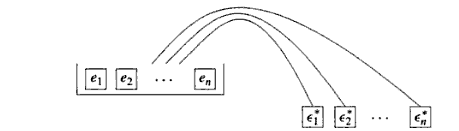
\includegraphics[width=8cm]{bs_reg.png}  
}

\frame{
	\frametitle{Regression Models}
        \begin{itemize}
          \item We draw $n $ times at random with replacement from
            this population to get bootstrap errors
            $\epsilon^*_1,\ldots \epsilon^*_n$. These are IID (because
            you sample them that way).
          \item Next we generate the $Y^*_i$:'
$$Y^* = X \hat \beta + \epsilon^*$$
\item  With the $Y^*$ and $X$, we can directly examine the
  distribution of $\hat \beta^*$, where $\hat
  \beta^*=(X'X)^{-1}X'Y^*$.
\item Note that this is known as the ``parametric'' bootstrap. 
\item The distribution of $\hat \beta^* - \hat \beta$ is a good
  approximation for the distribution of $\hat \beta - \beta$. In
  addition, the empirical covariance matrix of the $\hat \beta^*$ is a
  good approximation to the thoretical covariance matrix of $\hat \beta$.

        \end{itemize}
     
}




\end{document}
